% Sección VII: Integración de la solución, aplicación web y visualización
% evidencia:E20,E21,E22,E23,E28

\section{Integración de la solución, aplicación web y visualización}

MediFlow desacopla la extracción agregada sobre PostgreSQL respecto del servicio HTTP, la interfaz React y el tablero Power BI, impidiendo que el despliegue web acceda a la base hospitalaria o archivos Parquet en producción~\cite{mediflow2026informe}.

\subsection{Arquitectura modular y contratos HTTP de la API}

La Fig.~\ref{fig:arquitectura_tikz} esquematiza las capas reales: desde PostgreSQL de solo lectura, las consultas SQL \texttt{00}--\texttt{23} alimentan tanto el paquete Python \texttt{hun} (junto con \texttt{src/external/}) para producir \texttt{models/modelos\_web\_bundle.joblib} servido por FastAPI y React/Vite, como \texttt{preparar\_modelo.py} para generar el modelo estrella de Power BI PBIP~\cite{mediflow2026informe,mediflow2026pbip}.

\begin{figure*}[t]
\centering
\resizebox{\textwidth}{!}{%
\begin{tikzpicture}[
  node distance=6mm and 7mm,
  box/.style={draw=black!75, rounded corners=2pt, align=center, inner sep=4.5pt, minimum height=8.5mm, font=\footnotesize},
  priv/.style={box, fill=black!5},
  prod/.style={box, fill=black!10, thick},
  ext/.style={box, dashed},
  arr/.style={-{Stealth[length=2.1mm]}, semithick}
]
  \node[priv] (pg) {PostgreSQL HUN\\(OMOP solo lectura, VPN)};
  \node[priv, right=of pg] (sql) {SQL \texttt{00}--\texttt{23}\\Agregados \texttt{data/raw/}};
  \node[ext, below=of sql] (extd) {\texttt{src/external/}\\Calendario, clima, SIVIGILA};
  \node[priv, right=of sql] (hun) {Paquete \texttt{hun}\\Entrenamiento y empaquetado};
  \node[prod, right=of hun] (bundle) {Bundle \texttt{v2.0}\\(\texttt{.joblib}, corte \texttt{2026-07-17})};
  \node[prod, below=of bundle] (api) {API FastAPI\\15 rutas HTTP\\(\texttt{HUN\_MODO\_PRODUCCION=1})};
  \node[prod, left=of api] (web) {Frontend React / Vite\\5 vistas + simulador};
  \node[ext, below=of api] (chat) {\texttt{POST /api/chat}\\6 herramientas + respaldo};
  \node[priv, above=of sql] (pbi_prep) {\texttt{preparar\_modelo.py}\\(corte \texttt{2026-04-30})};
  \node[box, right=of pbi_prep] (pbip) {Proyecto PBIP Power BI\\7 pág., 12 tab., 43 medidas};

  \draw[arr] (pg) -- (sql);
  \draw[arr] (sql) -- (hun);
  \draw[arr] (extd) -- (hun);
  \draw[arr] (hun) -- node[above, font=\scriptsize]{\tiny offline} (bundle);
  \draw[arr] (bundle) -- (api);
  \draw[arr] (api) -- (web);
  \draw[arr] (api) -- (chat);
  \draw[arr] (sql) -- (pbi_prep);
  \draw[arr] (pbi_prep) -- (pbip);
\end{tikzpicture}%
}
\caption{Esquema conceptual de la arquitectura implementada en MediFlow (elaborado desde \texttt{app/api/\_\_init\_\_.py}, \texttt{empaquetar.py} y \texttt{dashboards/powerbi/}). No incluye integraciones HIS en vivo.}
\label{fig:arquitectura_tikz}
\end{figure*}

La inspección de \texttt{app/api/\_\_init\_\_.py} y \texttt{app/api/chat.py} verifica \textbf{15 rutas HTTP reales} (inventario completo en Anexo~C): \texttt{GET} \texttt{/api/health} (no existe \texttt{/api/salud}), \texttt{/api/modelo}, \texttt{/api/servicios}, \texttt{/api/parametros}, \texttt{/api/turnos/\{servicio\}}, \texttt{/api/ocupacion}, \texttt{/api/cuellos-botella}, \texttt{/api/\allowbreak comparacion/\allowbreak \{servicio\}}, \texttt{/api/\allowbreak efectos-eventos/\allowbreak \{servicio\}}, \texttt{/api/\allowbreak largo-plazo/\allowbreak \{servicio\}}, \texttt{/api/optimizacion}; y \texttt{POST} \texttt{/api/predecir}, \texttt{/api/predecir-rango}, \texttt{/api/optimizacion/simular} y \texttt{/api/chat}. Las menciones previas a \texttt{/api/historico/llegadas}, \texttt{/api/historico/turnos} o \texttt{/api/salud} en \texttt{DEC-007} y \texttt{tests/README.md} están obsoletas.

Tres salvaguardas acotan el backend~\cite{mediflow2026auditoria}: (1) en modo estricto (\texttt{HUN\_MODO\_PRODUCCION=1} o \texttt{HUN\_ENV=production}), \texttt{predict.py} lee solo \texttt{modelos\_web\_bundle.joblib} (o \texttt{HUN\_BUNDLE\_PATH}) y devuelve HTTP \texttt{503} ante falla, sin consultar Parquet; (2) \texttt{RangoRequest} acepta 1--30 días sintácticamente sin implicar validación predictiva a 30 días (backtests operativos de 1--7 días), y \texttt{/api/ocupacion} mide demanda diaria relativa a $p_{75}/p_{90}$, no camas físicas; y (3) \texttt{ALLOWED\_ORIGINS} restringe CORS pero no autentica usuarios, y la interfaz React/Vite no opera de forma autónoma sin el servidor FastAPI.

\subsection{Asistente conversacional (\texttt{/api/chat}) y tablero Power BI (PBIP)}

\texttt{app/api/chat.py} restringe el asistente a \textbf{seis herramientas deterministas de solo lectura} (\texttt{predecir}, \texttt{predecir\_rango}, \texttt{simular\_escenario}, \texttt{efecto\_promedio\_evento}, \texttt{indicadores\_\allowbreak cuellos\_\allowbreak botella}, \texttt{recomendaciones\_\allowbreak optimizacion}), sin acceso SQL ni emisión de órdenes médicas, con filtro fuera de tema, límite de 20 solicitudes/min por cliente, \textit{timeout} de 12\,s y tope de 150 palabras. Configura el identificador \texttt{claude-haiku-5-5} vía \texttt{ANTHROPIC\_API\_KEY} y conmuta a respaldo determinista offline si falta clave o falla el proveedor~\cite{mediflow2026informe}.

En Power BI (\nolinkurl{dashboards/powerbi/HUN_CuellosBotella/}), \texttt{model.bim} y las páginas definen \textbf{12 tablas} (5 dimensiones, 6 hechos, \texttt{\_Medidas}), \textbf{18 relaciones}, \textbf{43 medidas DAX} y \textbf{7 páginas} con \texttt{FechaCorte = 2026-04-30}~\cite{mediflow2026pbip}. Durante el cierre de auditoría se corrigieron textos locales en visuales (\texttt{esperasv12}, \texttt{hallazgosv02}, \texttt{hallazgosv03}, \texttt{metodologiav02}, \texttt{metodologiav03}) para evitar equiparar marcas OMOP con espera por cama; sin embargo, el PBIP no contiene datos y el enlace público no ha sido verificado ni republicado tras dichas ediciones~\cite{mediflow2026auditoria}. Persiste además la discrepancia entre \texttt{dashboards/README.md} (indica mayo de 2026 incompleto) e \texttt{inventario\_base.md} (sin meses vacíos hasta junio de 2026).

\subsection{Lectura crítica de las capturas archivadas de la interfaz}

Las Figs.~\ref{fig:app_cuellos}--\ref{fig:app_dashboard} documentan la interfaz React/Vite/Tailwind como \textbf{evidencia visual archivada} previa al cierre documental~\cite{mediflow2026informe}:
\begin{itemize}[leftmargin=*,nosep]
\item \textit{Cuellos de botella} (Fig.~\ref{fig:app_cuellos}): muestra censo mediano histórico en Hospitalización (283 frente a $p_{75}=297$ y $p_{90}=309$), matriz de turnos en Urgencias y barras $p_{90}$ de duración (\textit{Inpatient Visit} 188,2\,h).
\item \textit{Precisión histórica y asistente} (Fig.~\ref{fig:app_precision}): exhibe métricas del \textbf{modelo cuantílico servido} sobre 182 días en Urgencias (exactitud 91,1\,\%, WAPE 8,9\,\%, MAE 39,5\,pac./día, cobertura 78,6\,\%), no las del experimento Poisson (8,4\,\% WAPE).
\item \textit{Simulador de optimización} (Fig.~\ref{fig:app_simulador}): \textbf{imagen compuesta} de tres secciones verticales con rótulos de una versión anterior («Etapa 1 [Activa]», «Sin fuga de datos» y Little híbrido de 284); el código vigente separa el modo histórico del modo por corte y reporta ausencia de perfiles en \texttt{v2.0}.
\item \textit{Panel de pronóstico} (Fig.~\ref{fig:app_dashboard}): presenta un artefacto visual donde los siete días del 10 al 16 de julio de 2026 aparecen rotulados como festivos y etiquetas superpuestas en el eje horizontal de largo plazo; solo ilustra diseño general.
\end{itemize}

\begin{figure*}[t]
\centering
\begin{minipage}[t]{0.48\textwidth}
\centering
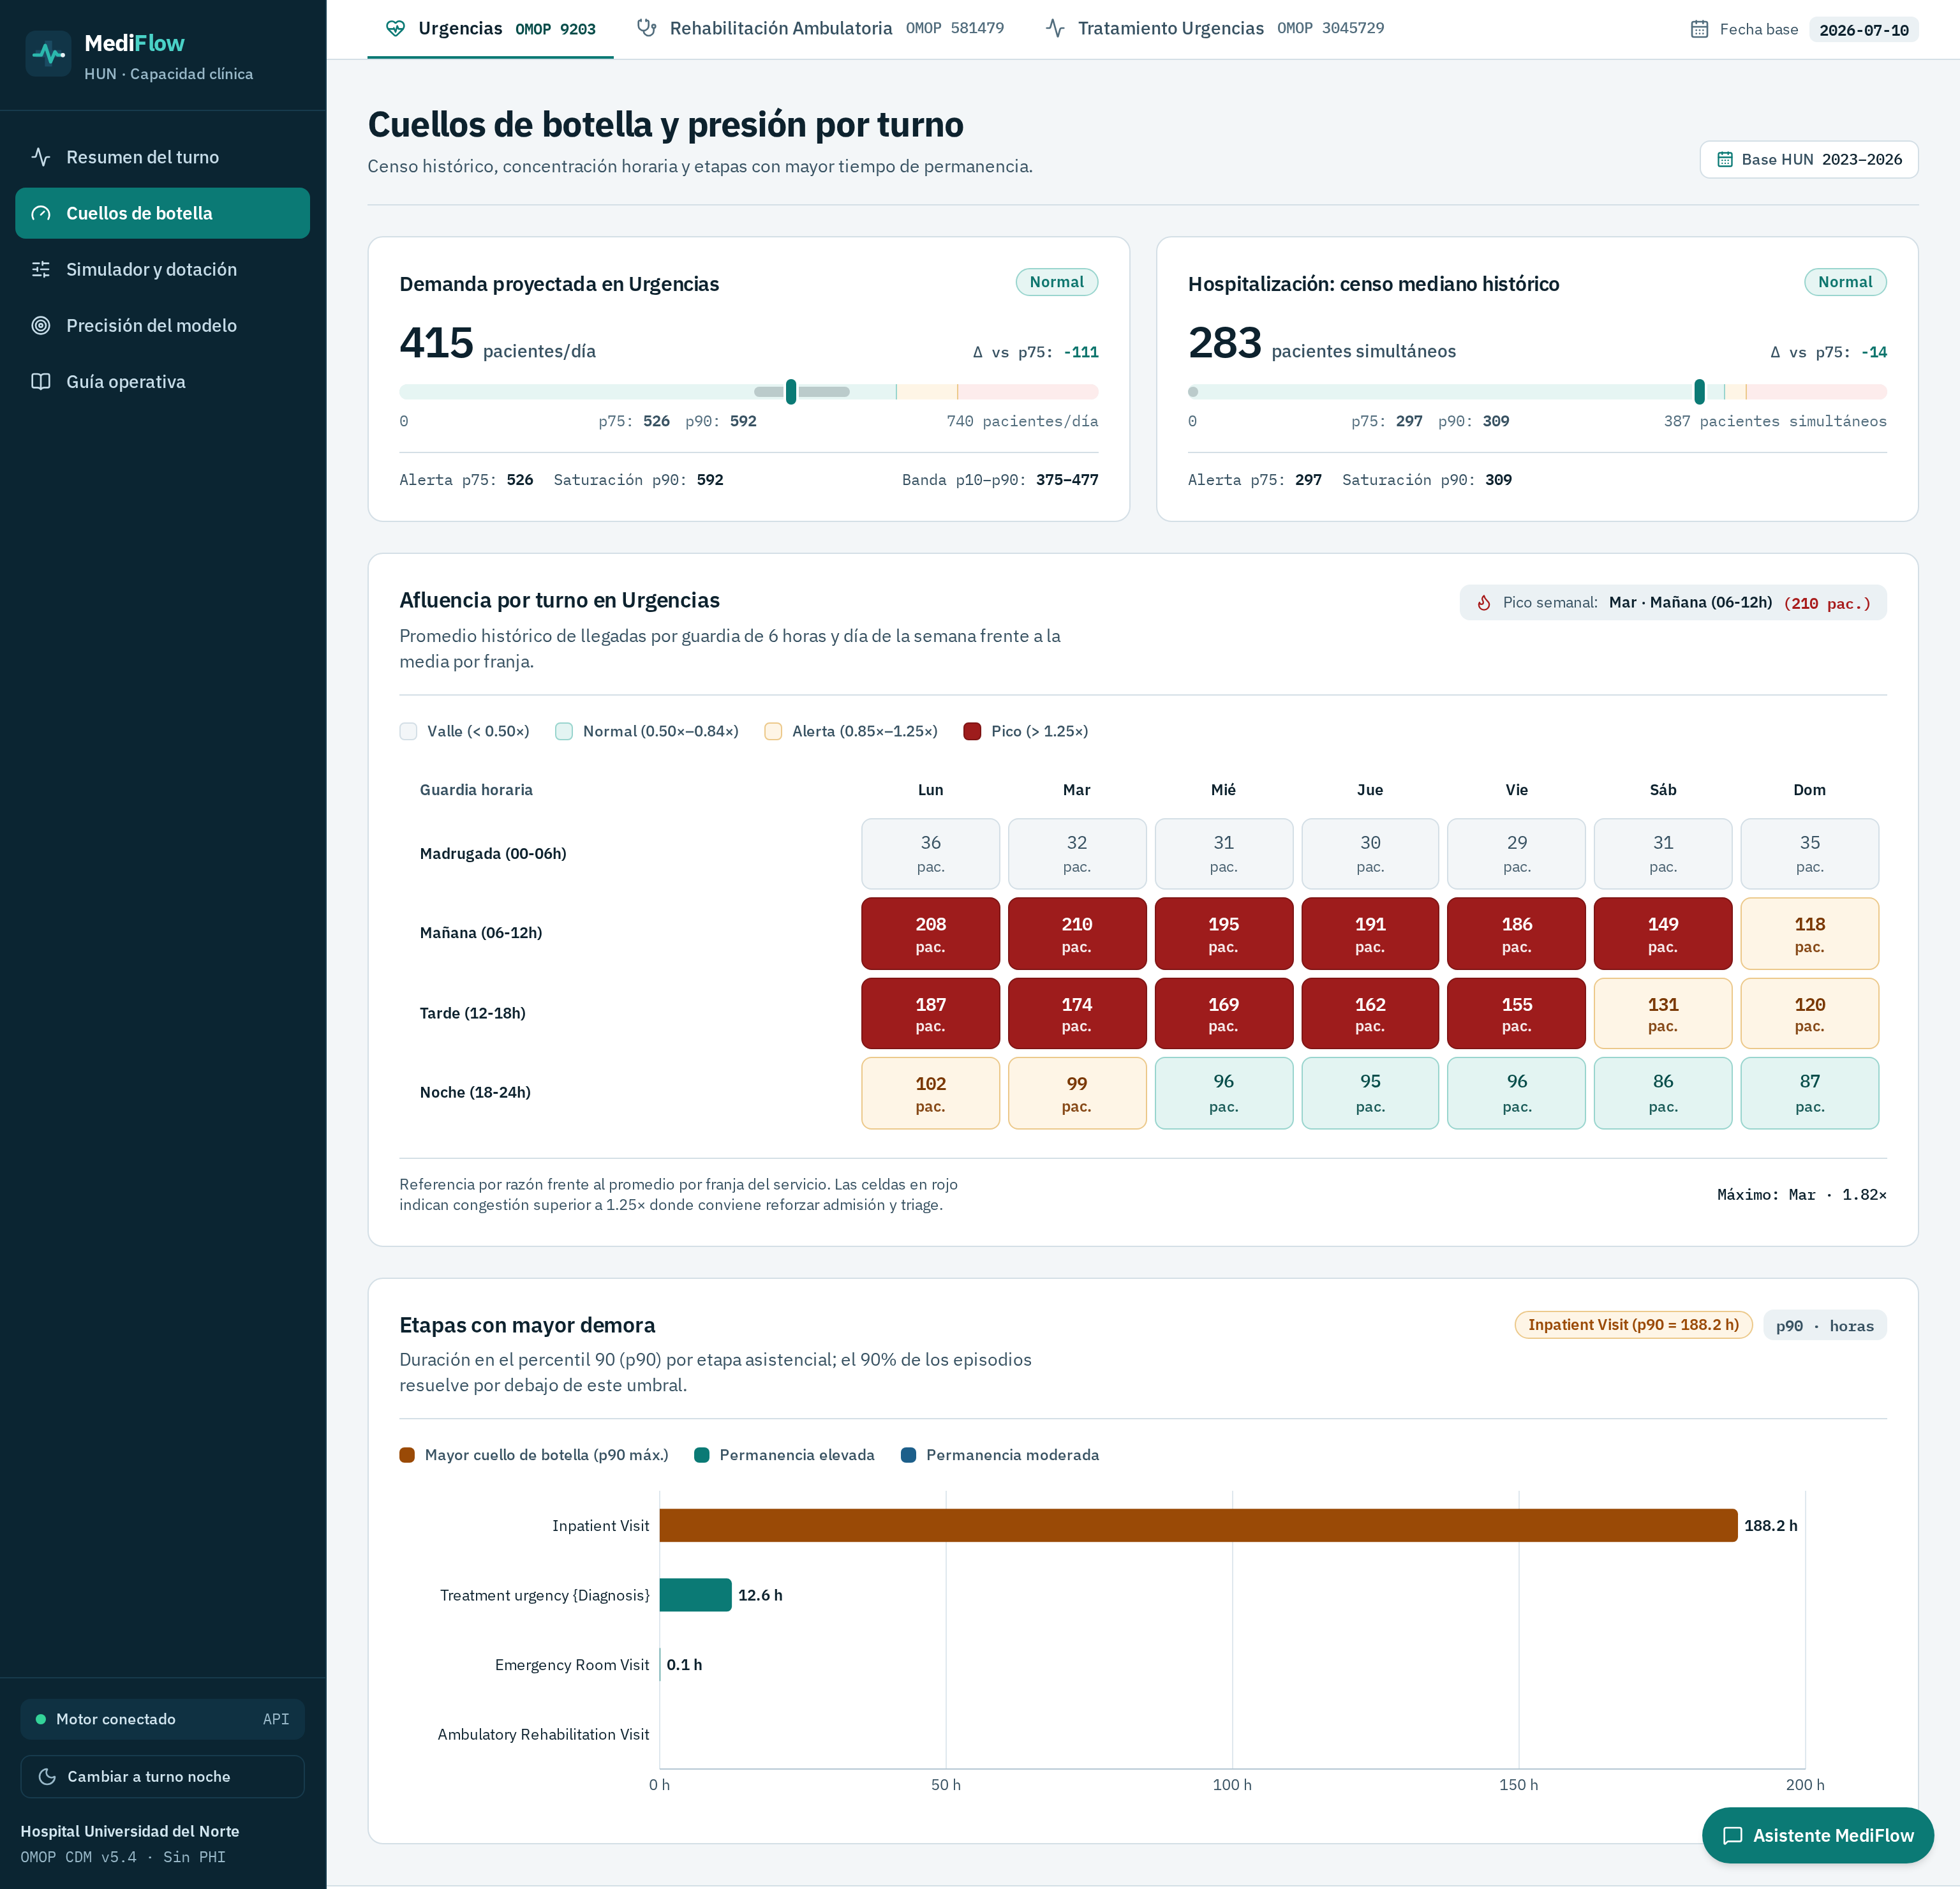
\includegraphics[width=\textwidth,height=0.38\textheight,keepaspectratio]{cuellos_botella.png}
\caption{Vista archivada de cuellos de botella y presión por turno (\protect\nolinkurl{cuellos_botella.png}). No representa ejecución en vivo ni camas habilitadas.}
\label{fig:app_cuellos}
\end{minipage}\hfill
\begin{minipage}[t]{0.48\textwidth}
\centering
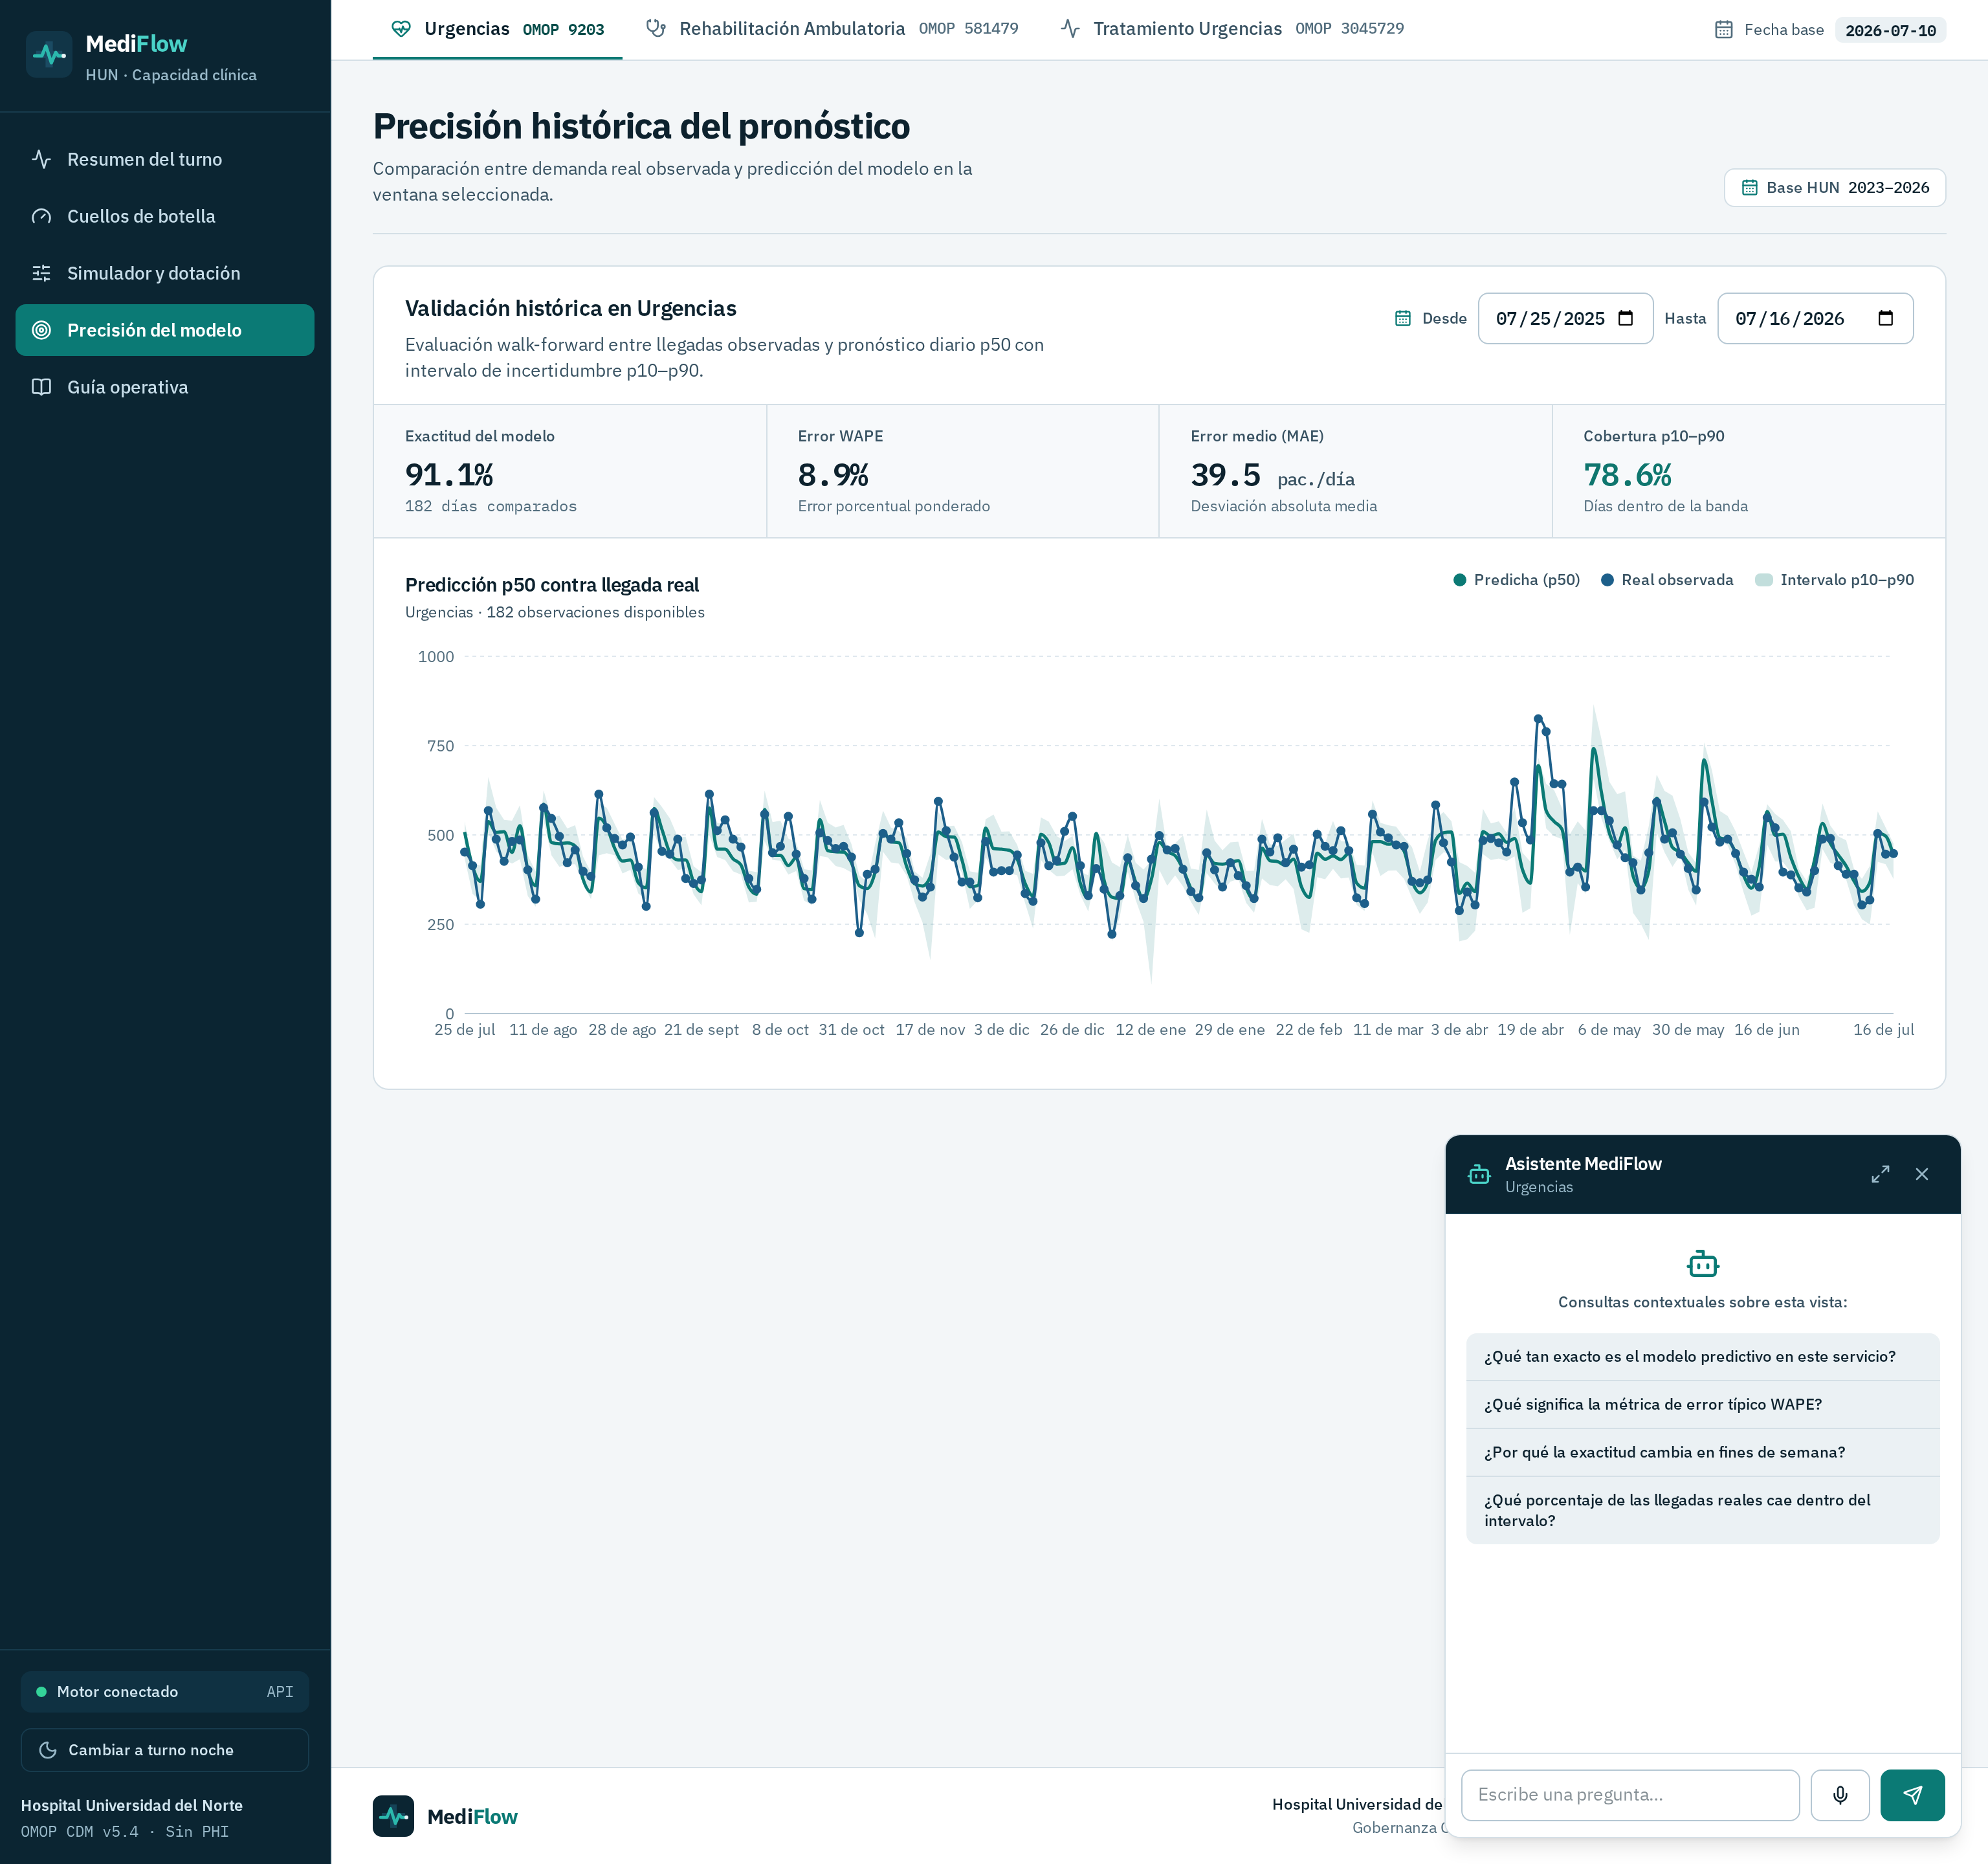
\includegraphics[width=\textwidth,height=0.38\textheight,keepaspectratio]{precision_asistente.png}
\caption{Vista archivada de precisión histórica en Urgencias con asistente (\protect\nolinkurl{precision_asistente.png}). Corresponde al bundle cuantílico \texttt{v2.0} (182\,d).}
\label{fig:app_precision}
\end{minipage}
\end{figure*}

\begin{figure*}[t]
\centering
\begin{minipage}[t]{0.48\textwidth}
\centering
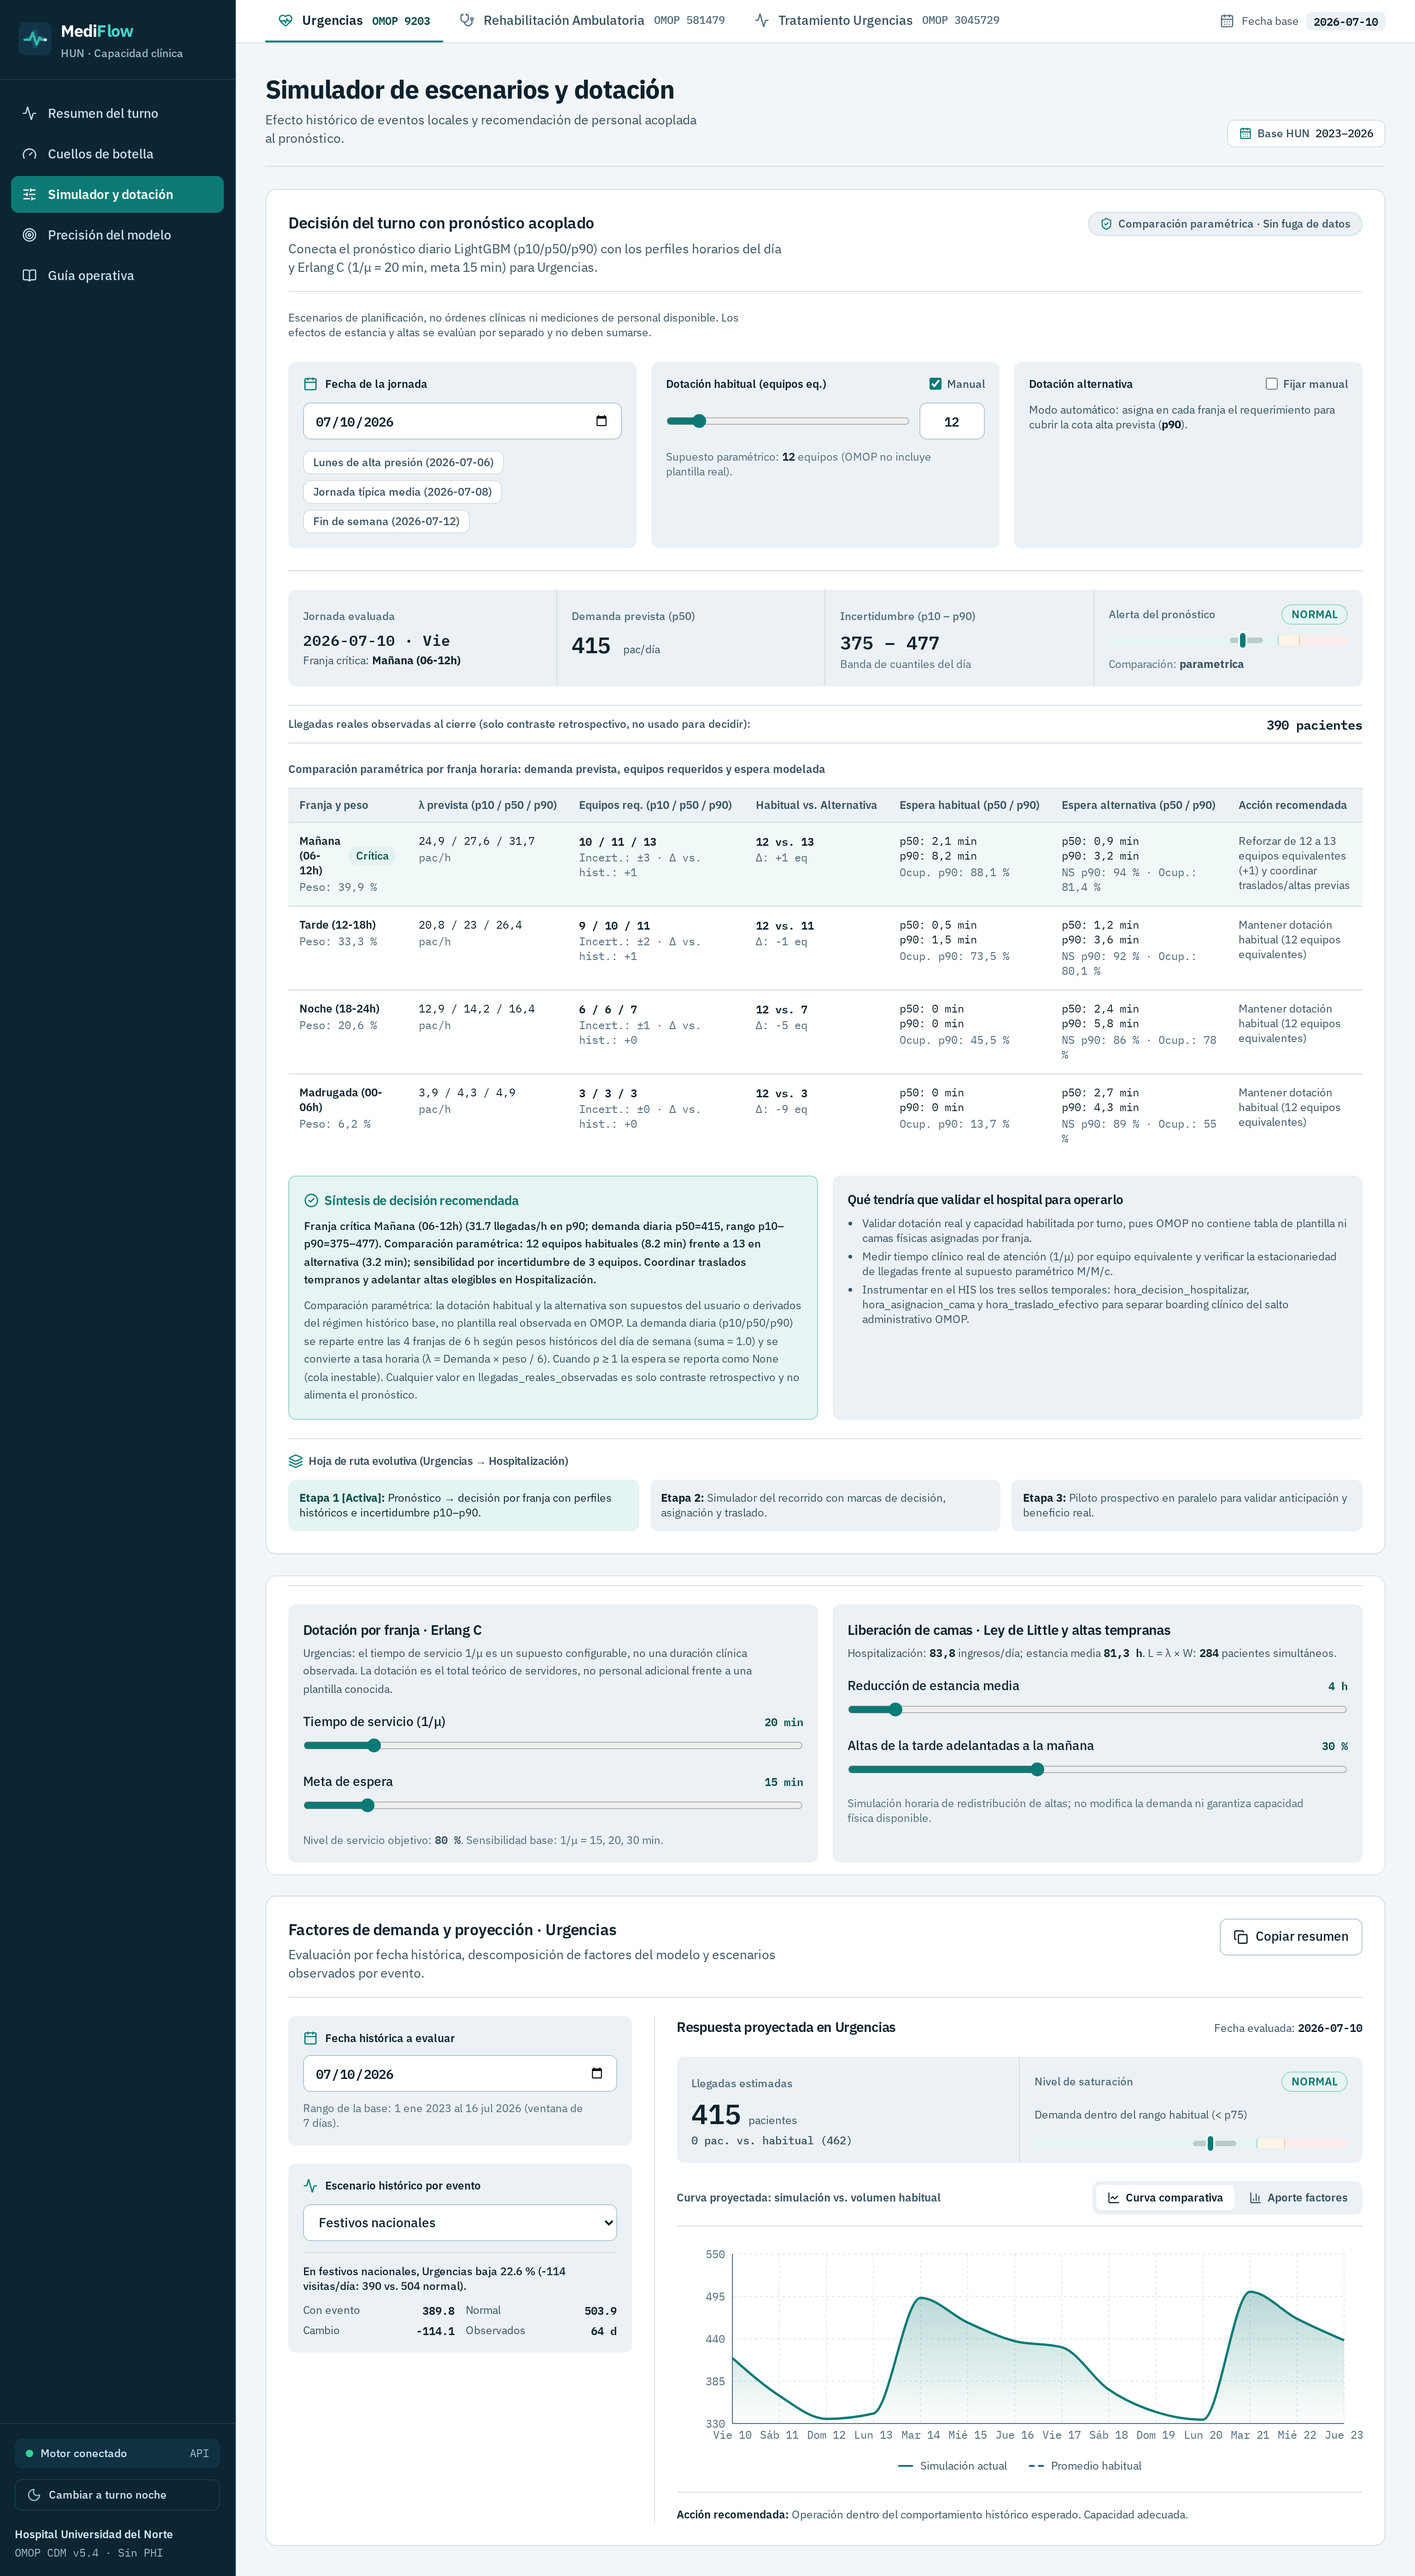
\includegraphics[width=\textwidth,height=0.46\textheight,keepaspectratio]{simulador_optimizacion.png}
\caption{Captura compuesta archivada del simulador (\protect\nolinkurl{simulador_optimizacion.png}). Conserva rótulos previos («Etapa 1 [Activa]», Little 284).}
\label{fig:app_simulador}
\end{minipage}\hfill
\begin{minipage}[t]{0.48\textwidth}
\centering
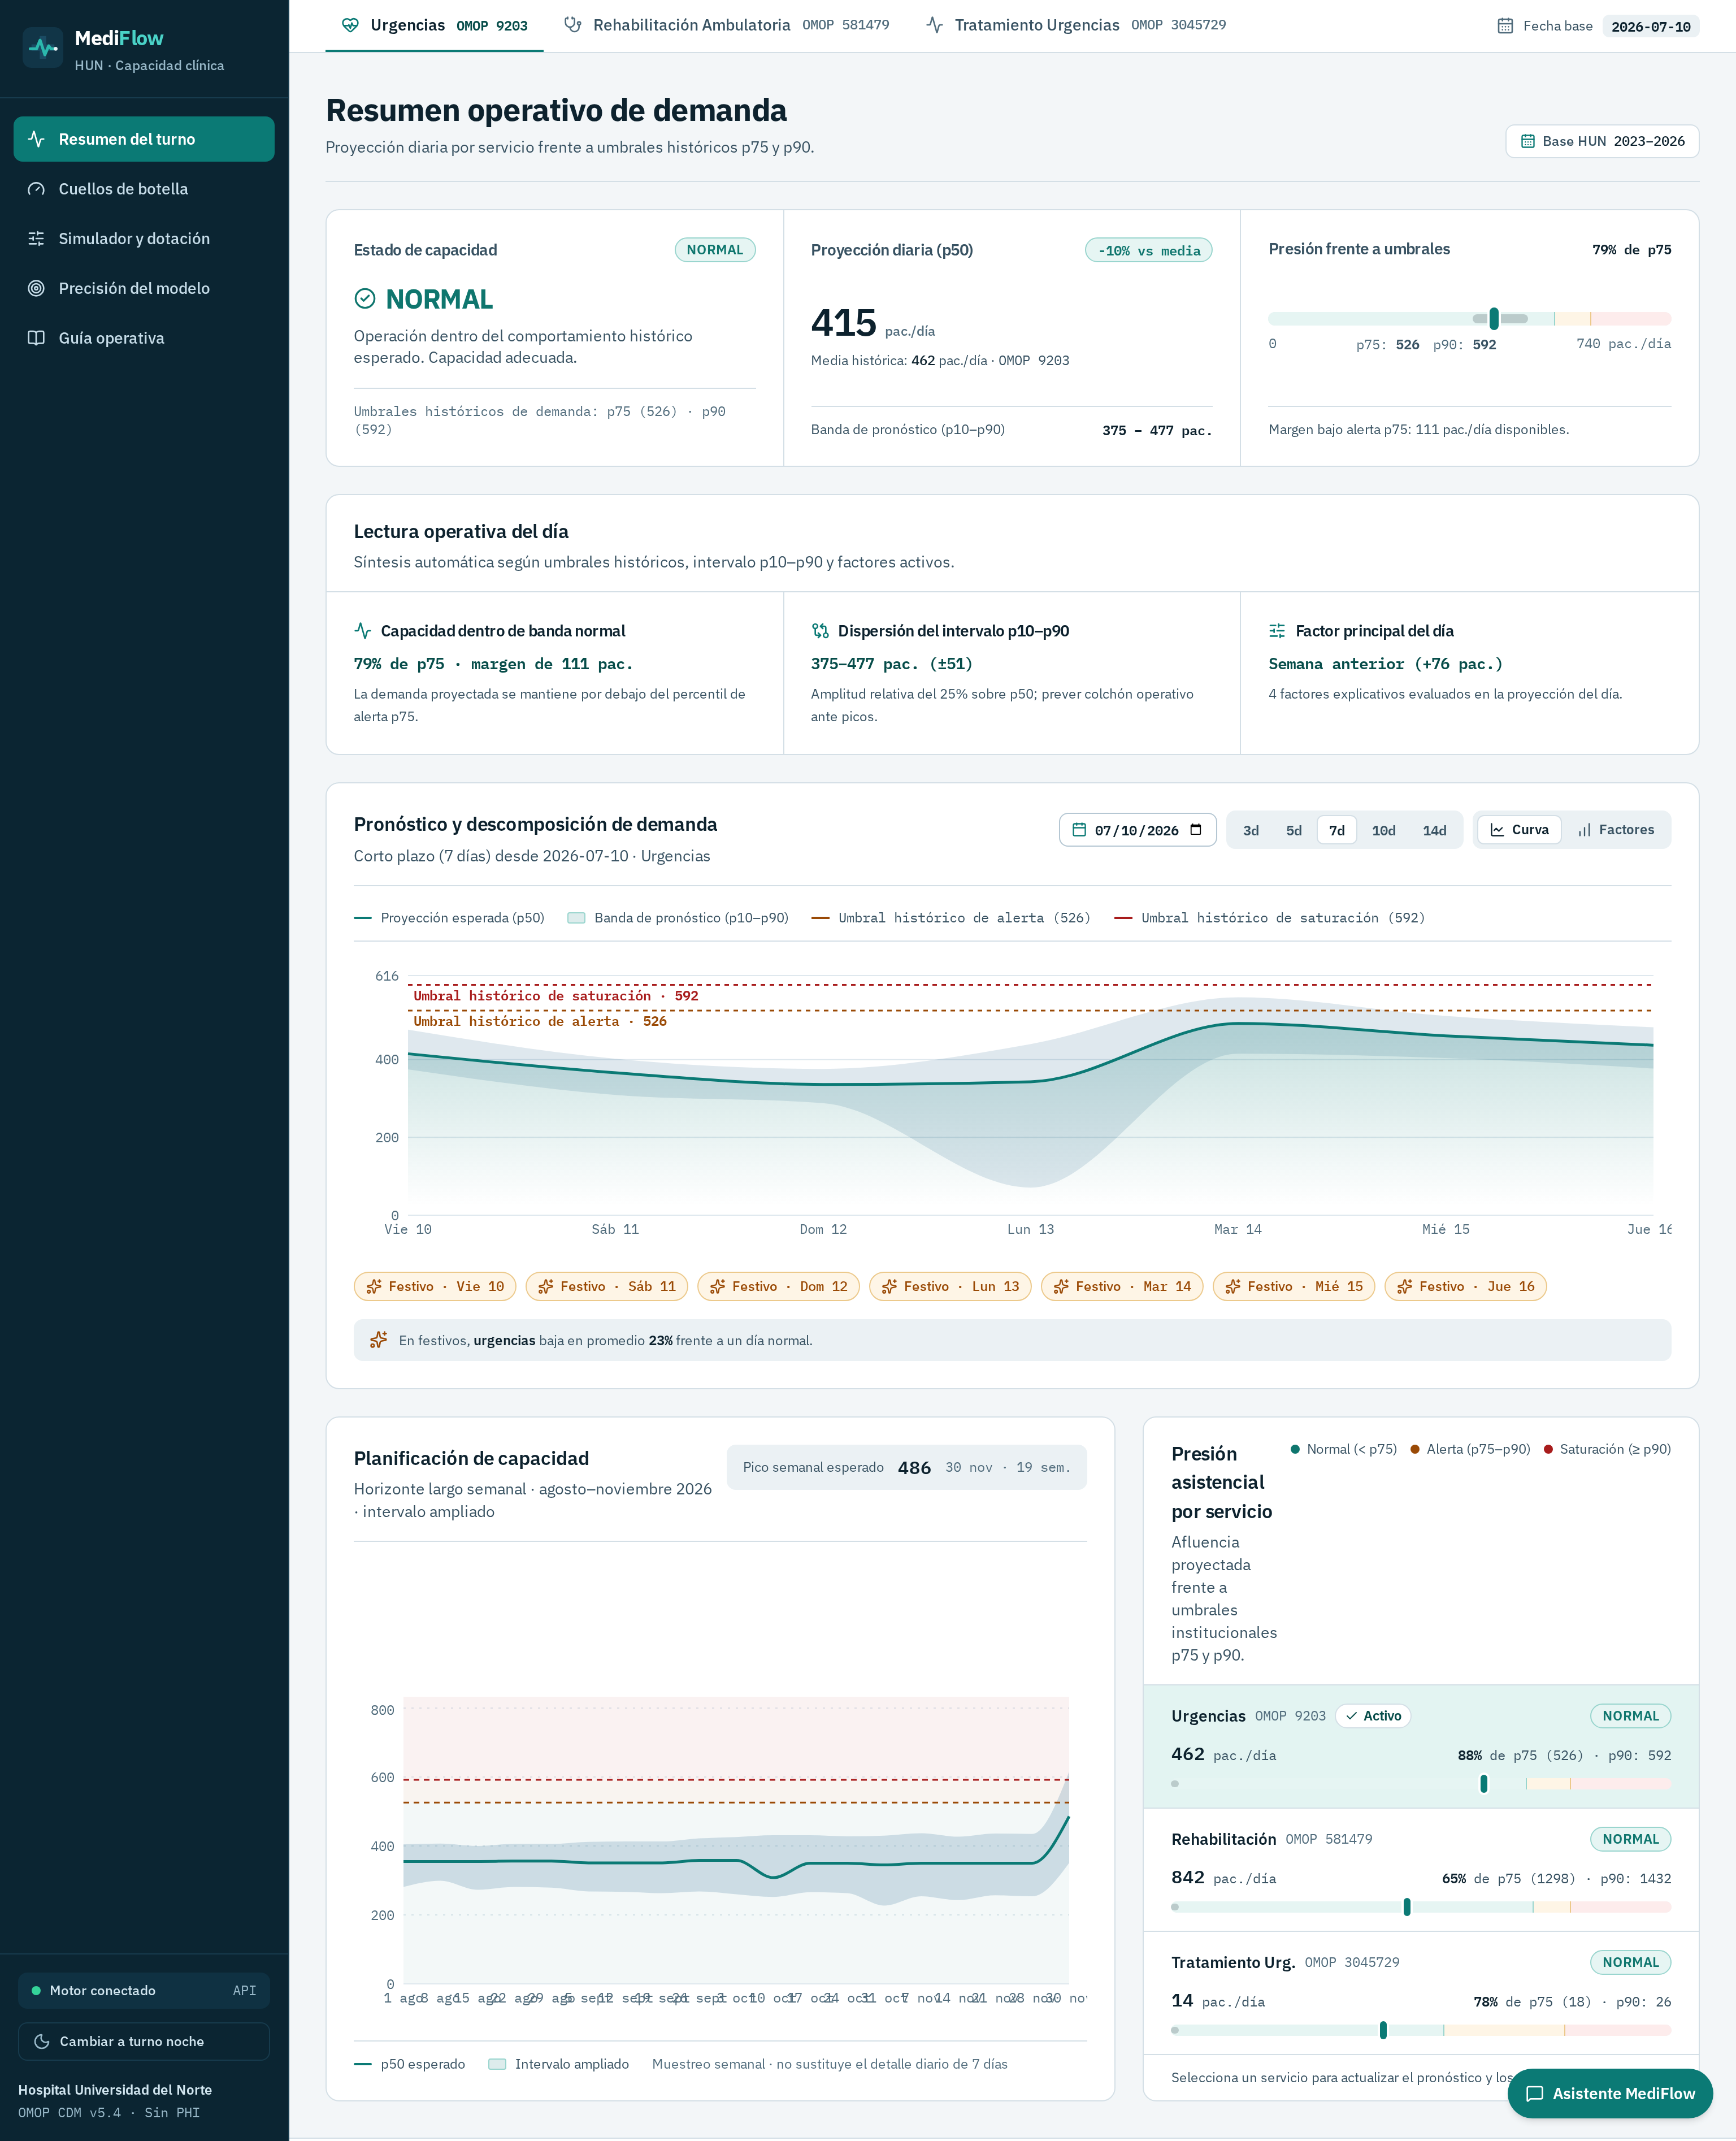
\includegraphics[width=\textwidth,height=0.46\textheight,keepaspectratio]{dashboard_pronostico.png}
\caption{Vista archivada del tablero de pronóstico (\protect\nolinkurl{dashboard_pronostico.png}). Advertencia: rotula «Festivo» del 10 al 16 de julio y superpone ejes.}
\label{fig:app_dashboard}
\end{minipage}
\end{figure*}

\FloatBarrier
